\documentclass{anstrans}
%%%%%%%%%%%%%%%%%%%%%%%%%%%%%%%%%%%
\title{Validation of Spent Nuclear Fuel Output by Cyclus, a Fuel Cycle Simulator Code}
\author{Gwendolyn J. Chee, Gyutae Park, and Kathryn D. Huff}

\institute{
Dept. of Nuclear, Plasma and Radiological Engineering, University of Illinois at Urbana-Champaign \\
gchee2@illinois.edu
}

%%%% packages and definitions (optional)
\usepackage{graphicx} % allows inclusion of graphics
\usepackage{booktabs} % nice rules (thick lines) for tables
\usepackage{microtype} % improves typography for PDF
\usepackage{xspace}
\usepackage{tabularx}
\usepackage{subcaption}
\newcommand{\SN}{S$_N$}
\renewcommand{\vec}[1]{\bm{#1}} %vector is bold italic
\newcommand{\vd}{\bm{\cdot}} % slightly bold vector dot
\newcommand{\grad}{\vec{\nabla}} % gradient
\newcommand{\ud}{\mathop{}\!\mathrm{d}} % upright derivative symbol
\newcommand{\Cyclus}{\textsc{Cyclus}\xspace}%
\newcommand{\Cycamore}{\textsc{Cycamore}\xspace}%
\newcolumntype{c}{>{\hsize=.56\hsize}X}
\newcolumntype{b}{>{\hsize=.7\hsize}X}
\newcolumntype{s}{>{\hsize=.74\hsize}X}
\newcolumntype{f}{>{\hsize=.1\hsize}X}
\newcolumntype{a}{>{\hsize=.45\hsize}X}
\usepackage{titlesec}
\titleformat*{\subsection}{\normalfont}

\begin{document}
%%%%%%%%%%%%%%%%%%%%%%%%%%%%%%%%%%%%%%%%%%%%%%%%%%%%%%%%%%%%%%%%%%%%%%%%%%%%%%%%
\section{Introduction}
\Cyclus \cite{carlsen_cyclus_2014}, a fuel cycle simulator, was used to simulate the
United States' nuclear fuel cycle from 1967 through 2013. The \Cyclus spent nuclear fuel (SNF) inventory was compared to SNF inventory from the U.S Department of Energy (DOE) sponsored Unified Database (UDB) \cite{peterson_unf-st&dards_2017}. The UDB provides comprehensive and consistent technical data on reactor sites and spent nuclear fuel (SNF) from the beginning of nuclear reactor operation in the United States until 2013. This comparison between \Cyclus and UDB establishes a realistic validation of \Cyclus capabilities to produce accurate isotopic compositions and total spent fuel mass that closely match reality. 

%%% 
\section{Background}
\Cyclus is an agent-based fuel cycle simulation framework \cite{huff_fundamental_2016}, which means that each facility in the fuel cycle is modeled as an agent. \Cycamore \cite{carlsen_cycamore_2014} provides agents to represent process physics of various components of the nuclear fuel cycle (e.g. mine, fuel enrichment facility, reactor) \cite{huff_extensions_2014}. 

%%%%%%%%%%%%%%%%%%%%%%%%%%%%%%%%%%%%%%%%%%%%%%%%%%%%%%%%%%%%%%%%%%%%%%%%%%%%%%%%
\section{Motivation}
The United States is currently considering various fuel cycles and geologic disposal options
\cite{DOE_strategy_2013}. Decisions such as waste package spacing, waste repository size and geometry will be influenced by key criteria such as thermal load of waste packages and the thermal capacity of the selected geologic host media. Waste package thermal evolution depends on the decay heat contribution from each isotope in the spent fuel. Therefore, to correctly simulate loading of a waste repository based on thermal constraints in \Cyclus, the simulation must first give isotopic composition and spent fuel mass that closely replicate reality. 

%%%%%%%%%%%%%%%%%%%%%%%%%%%%%%%%%%%%%%%%%%%%%%%%%%%%%%%%%%%%%%%%%%%%%%%%%%%%%%%%
\section{Methodology}
\subsection{\textit{Generating \Cyclus Simulation and Analysis}}
A \Cyclus simulation of the United States nuclear fuel cycle was created using published data about the 112 commerical nuclear reactors that have operated since 1967 in the United States. The reactor deployment data was obtained from the Power Reactor Information System (PRIS) reactor database \cite{IAEA_pris_2017}. The relevant data included the: country, reactor unit, type, net capacity (MWe), first grid date and shutdown date. Data for reactors in the United States were extracted and used to populate the simulation. The nuclear fuel in reactors in the simulation are recipe based, which means that input recipes specify mass fractions for each isotope for both fresh and spent fuel. The recipes are taken from a reference depletion calculation done using ORIGEN \cite{bell_origen_1973}. The recipes were also used in \cite{wilson_adoption_2009, bae_synergistic_2017}. 

Jinja2 \cite{ronacher_welcome_2018}, a Python templating language, was then used in Python to render the data into an input file that can be accepted by \Cyclus. The output file produced by \Cyclus was also analyzed using Python. 

The assumptions made for this \Cyclus simulation include: 

\begin{enumerate}
	\item Decay is not taken into account. 
	\item Cycle time is assumed to be 18 months. 
	\item Refuel time is assumed to be 1 month. 
\end{enumerate}


\subsection{\textit{UDB Data Analysis}}
The UDB data contained SNF information from 1967 up to 2013. The dataset includes discharged fuel assembly data per reactor, specific isotopic concentrations and decay heat for each assembly along with its discharge date \cite{peterson_unf-st&dards_2017}. The UDB dataset was imported into Python and processed to be compared with \Cyclus simulation output. All scripts and data used are available in \cite{chee_arfc/transition-scenarios_2018}. 
%%%%%%%%%%%%%%%%%%%%%%%%%%%%%%%%%%%%%%%%%%%%%%%%%%%%%%%%%%%%%%%%%%%%%%%%%%%%%%%%
\section{Results and Analysis}
The primary outcome of this validation is to provide comparisons between \Cyclus and UDB for spent fuel mass and major isotopic contributions to the total spent fuel mass. 

\subsection{\textit{Cumulative Total Spent Fuel Mass Comparison}}
Figure \ref{fig:total_original} shows the cumulative spent fuel mass for both \Cyclus and UDB data from 1967 to 2013. The total spent fuel mass estimated by \Cyclus is larger than UDB data before the year 2000 and diverge after, with UDB being larger. The discrepancies can be attributed to rigidity of \Cyclus simulation input with respect to cycle and refuel time. In \Cyclus, the user specifies refuel and cycle times for each reactor as constant integer months. In reality, the cycle and refuel times vary throughout each reactor's lifetime and are not exact integer multiples of one month. 

\begin{figure}[h] % replace 't' with 'b' to force it to be on the bottom
	\centering
	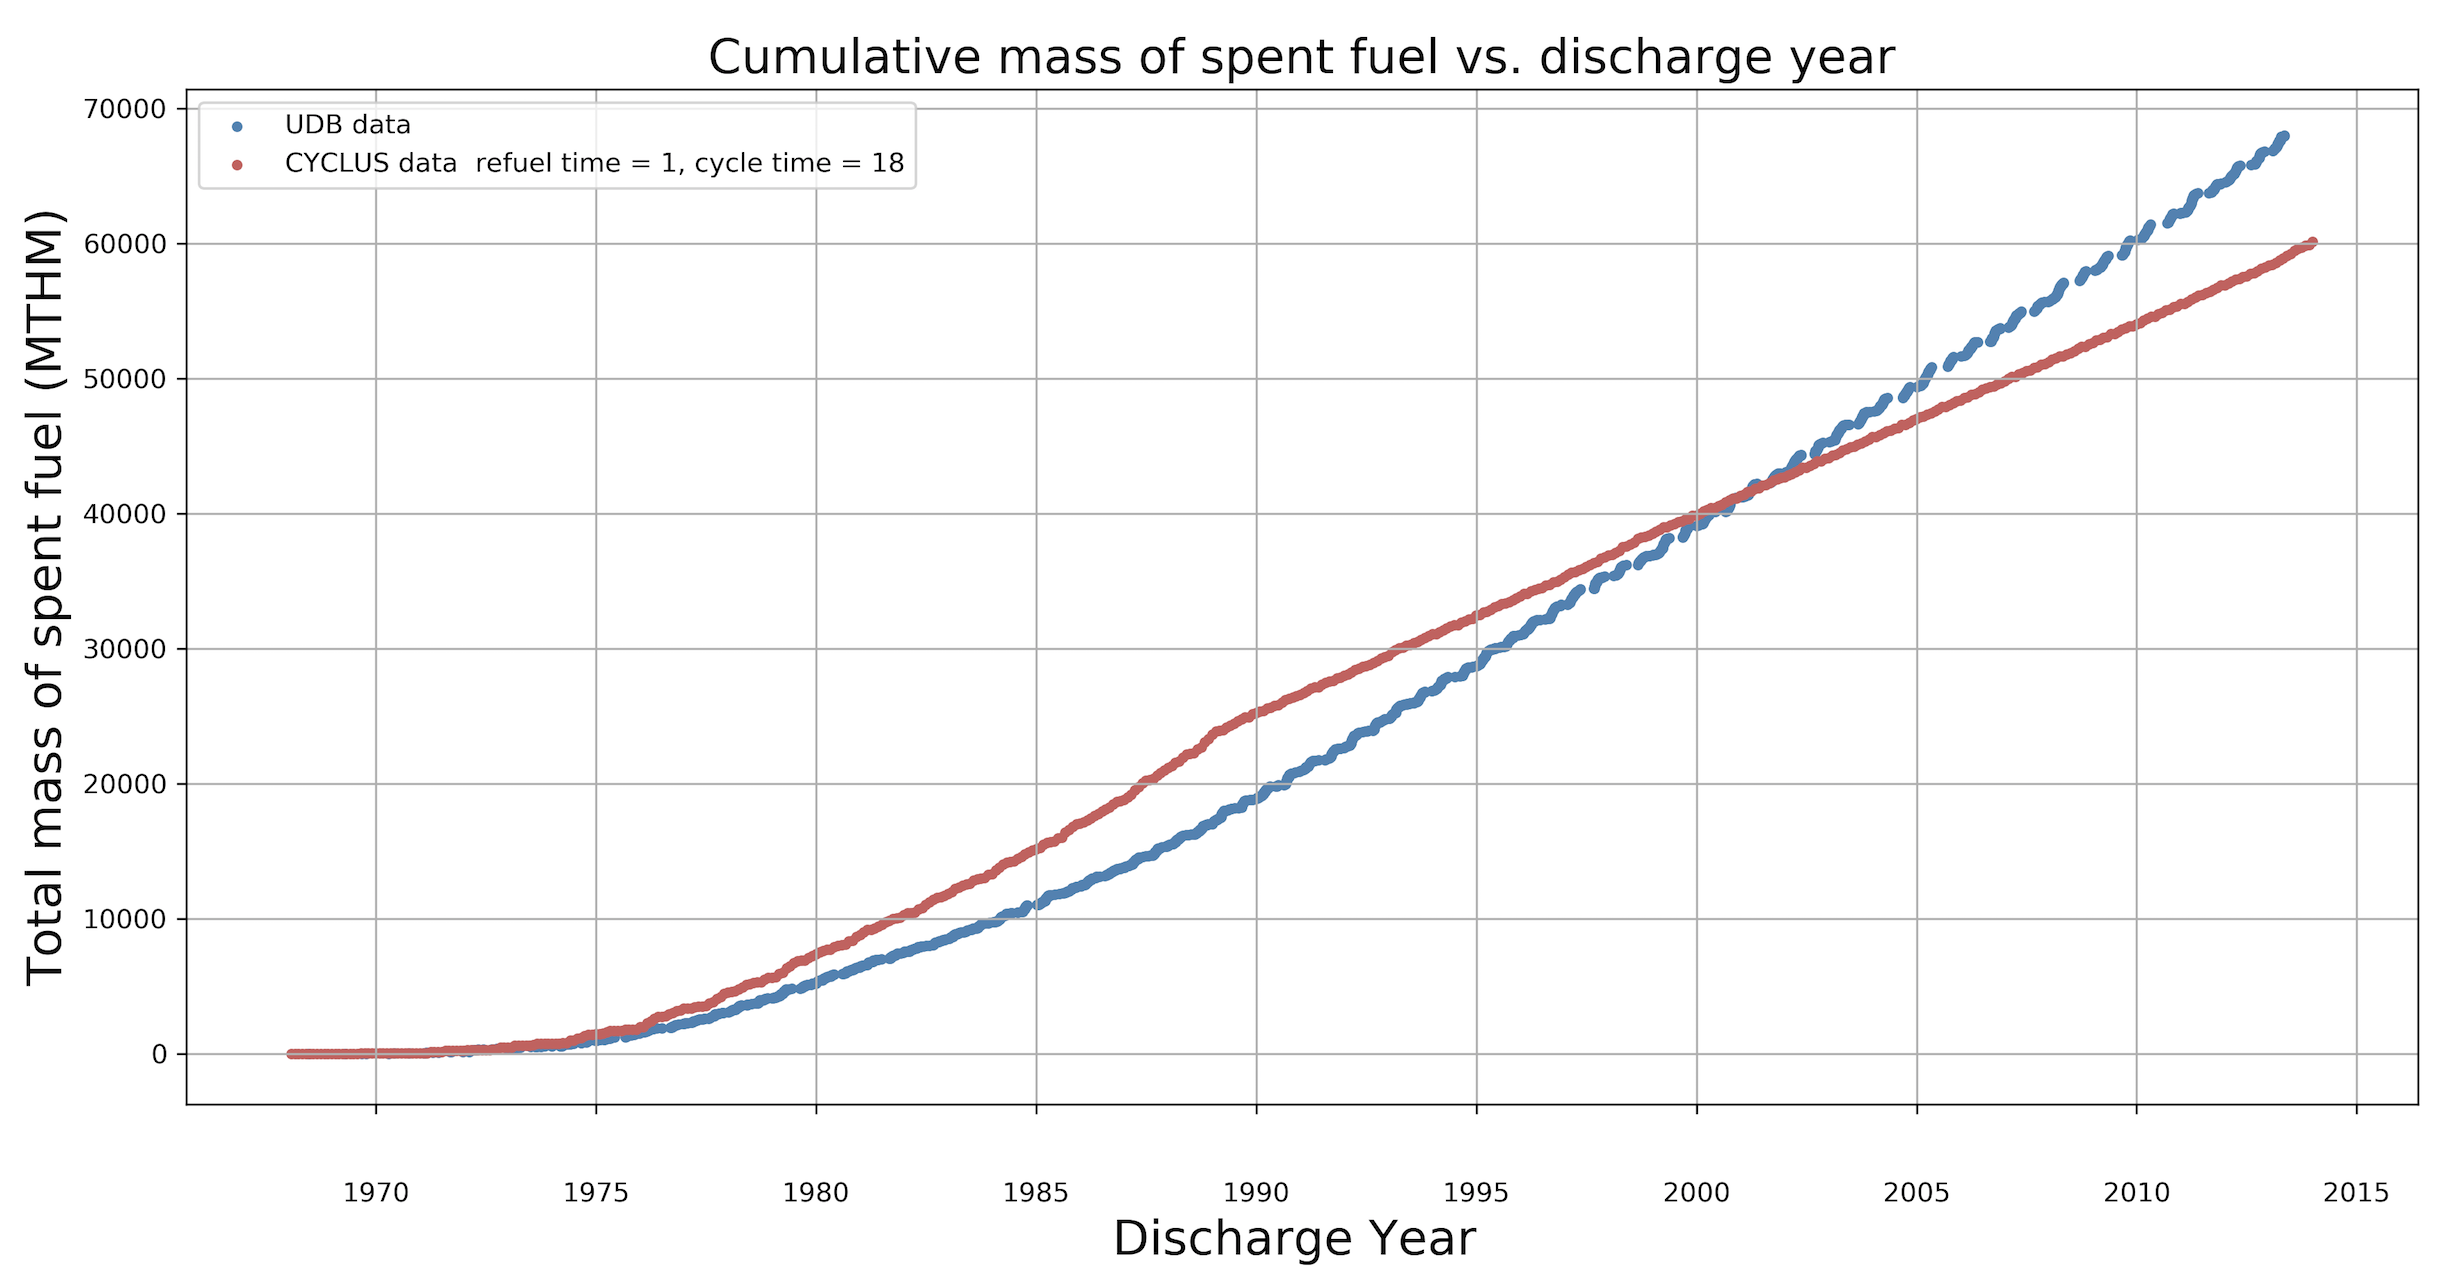
\includegraphics[width=0.48\textwidth]{total_cumulative_mass_spent_fuel_original}
	\caption{Total cumulative spent fuel mass against discharge time for \Cyclus and UDB data from 1967 up to 2013.}
	\label{fig:total_original}
\end{figure}

The Nuclear Energy Institute (NEI) reported that there has been significant variance in the refueling period for reactors in the United States. The average refuelling time in 1990 was 104 days, and generally decreased to an average refuelling time of 35 days in 2017 \cite{iaea_current_nodate}.

Figure \ref{fig:total_refueltime} includes plots of total spent fuel mass from \Cyclus simulations where refuel time is increased. A longer refuel time brings the total spent fuel mass from \Cyclus simulations closer to the UDB data before 2000. 

\begin{figure}[h] 
	\centering
	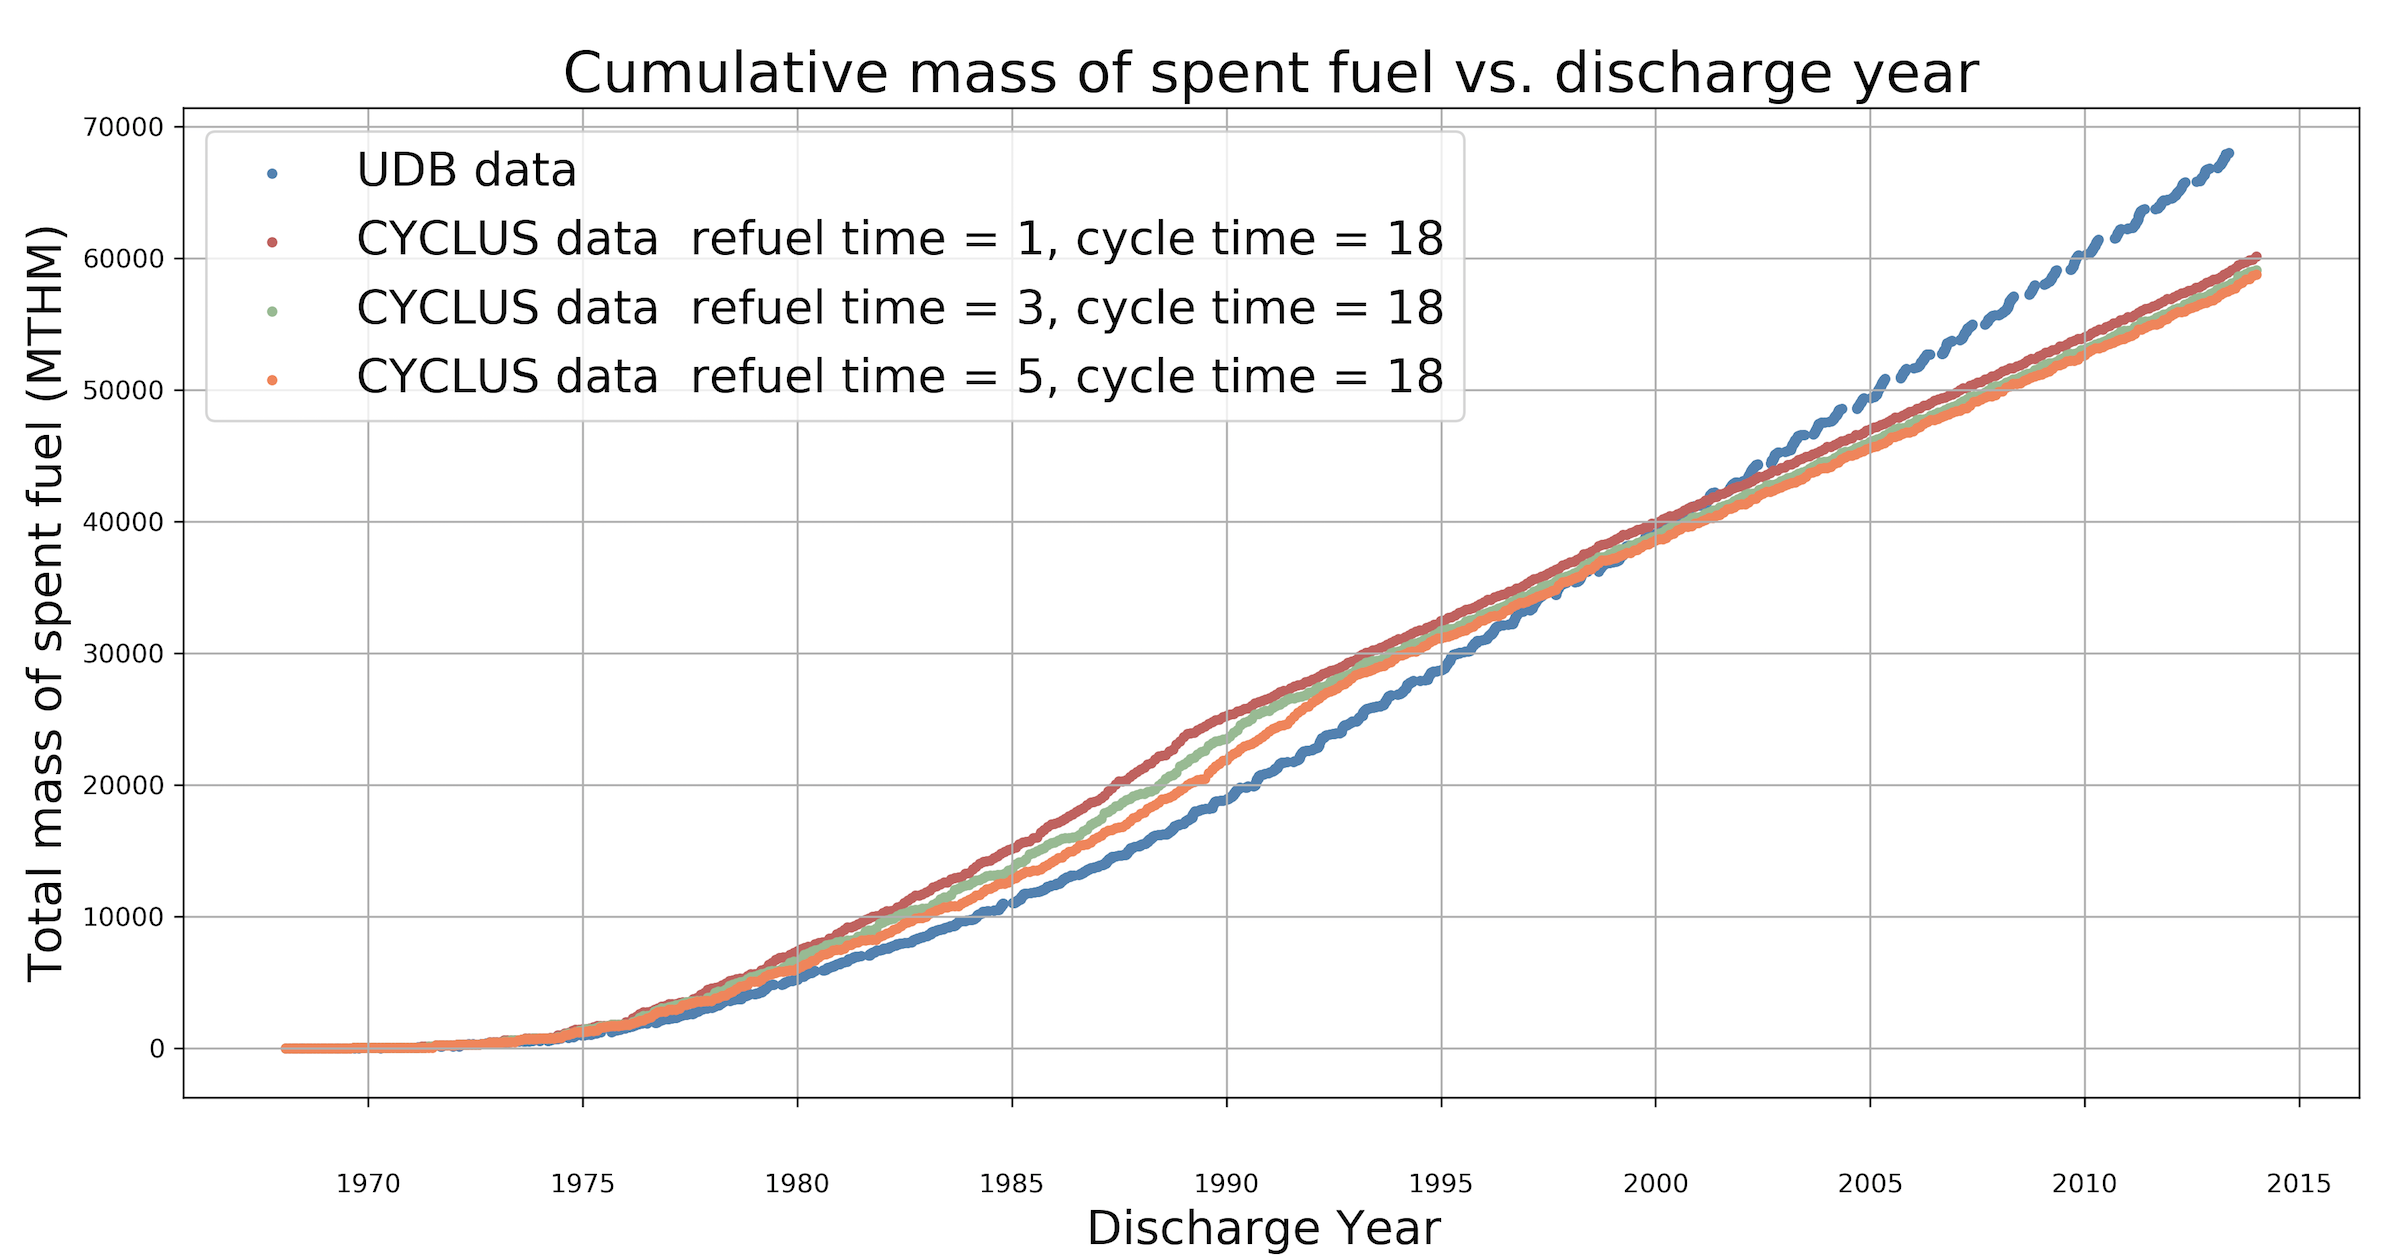
\includegraphics[width=0.48\textwidth]{total_cumulative_mass_spent_fuel_refueltime}
	\caption{Total cumulative spent fuel mass against discharge time for \Cyclus and UDB data from 1967 up to 2013 for varying refuel time}
	\label{fig:total_refueltime}
\end{figure} 

The larger cumulative UDB spent fuel mass compared to the \Cyclus simulation after 2000 can be attributed to the real world cycle lengths being shorter than the 18 month length of \Cyclus simulations. The United States DOE reported that there was a downward trend of forced outage rates of nuclear reactors from 2000 to 2014. The forced outage rate was 4.24\% in 2000 and 2.98\% in 2013 \cite{gehin_nuclear_2016}. As the rate of forced outages decreased from 2000 to 2013, the cycle length also decreased. 

Figure \ref{fig:total_cycletime} includes plots of total spent fuel mass from \Cyclus simulations where cycle time is varied. A shorter cycle time brings the total spent fuel mass from \Cyclus simulations closer to the UDB data after 2000. 

\begin{figure}[h] % replace 't' with 'b' to force it to be on the bottom
	\centering
	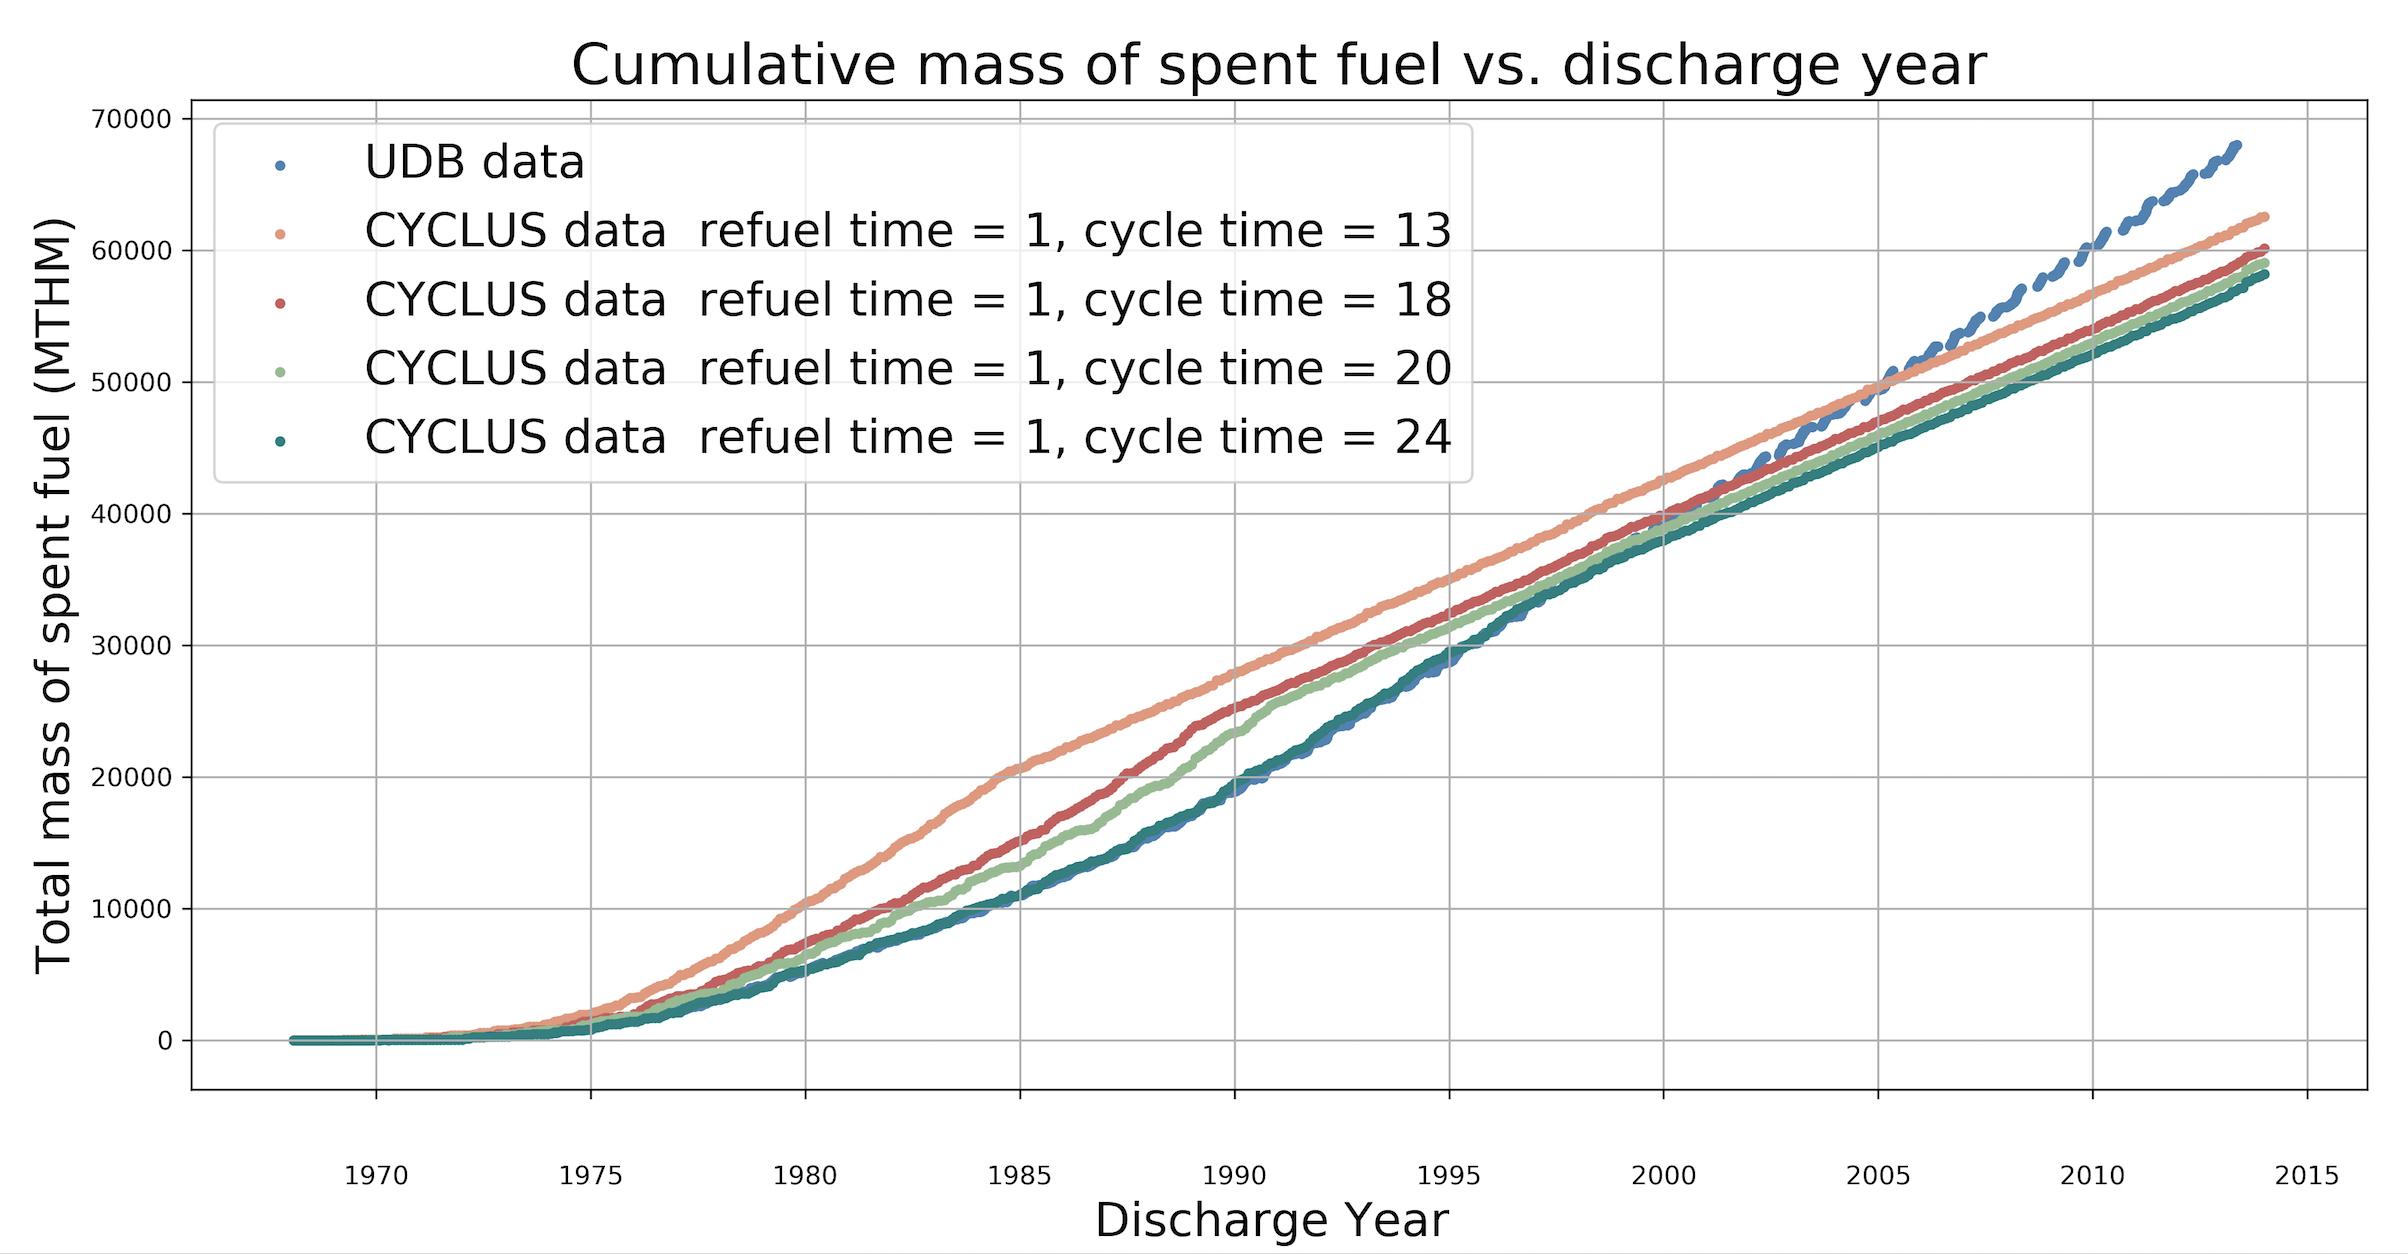
\includegraphics[width=0.48\textwidth]{total_cumulative_mass_spent_fuel_cycletime}
	\caption{Total cumulative spent fuel mass against discharge time for \Cyclus and UDB data from 1967 to 2013 for varying cycle time}
	\label{fig:total_cycletime}
\end{figure} 

\subsection{\textit{Major Isotopic Composition of  Spent Fuel Mass Comparison}}
The three isotopes that contribute the most to the total mass of the spent fuel, in order of significance, are: $^{238}$U, $^{235}$U, $^{239}$Pu.  

Figure \ref{fig:total_u238}, \ref{fig:total_u235} and \ref{fig:total_pu240} show the cumulative spent fuel mass for $^{238}$U, $^{235}$U and $^{239}$Pu isotopes for both \Cyclus and UDB data from 1967 to 2013.
The figures follow a similar trend as figure \ref{fig:total_original} and the same explanations can be used to explain the differences in masses before and after year 2000.  

\begin{figure}[h]
	\centering
	\begin{subfigure}[b]{0.45\textwidth}
		\centering
		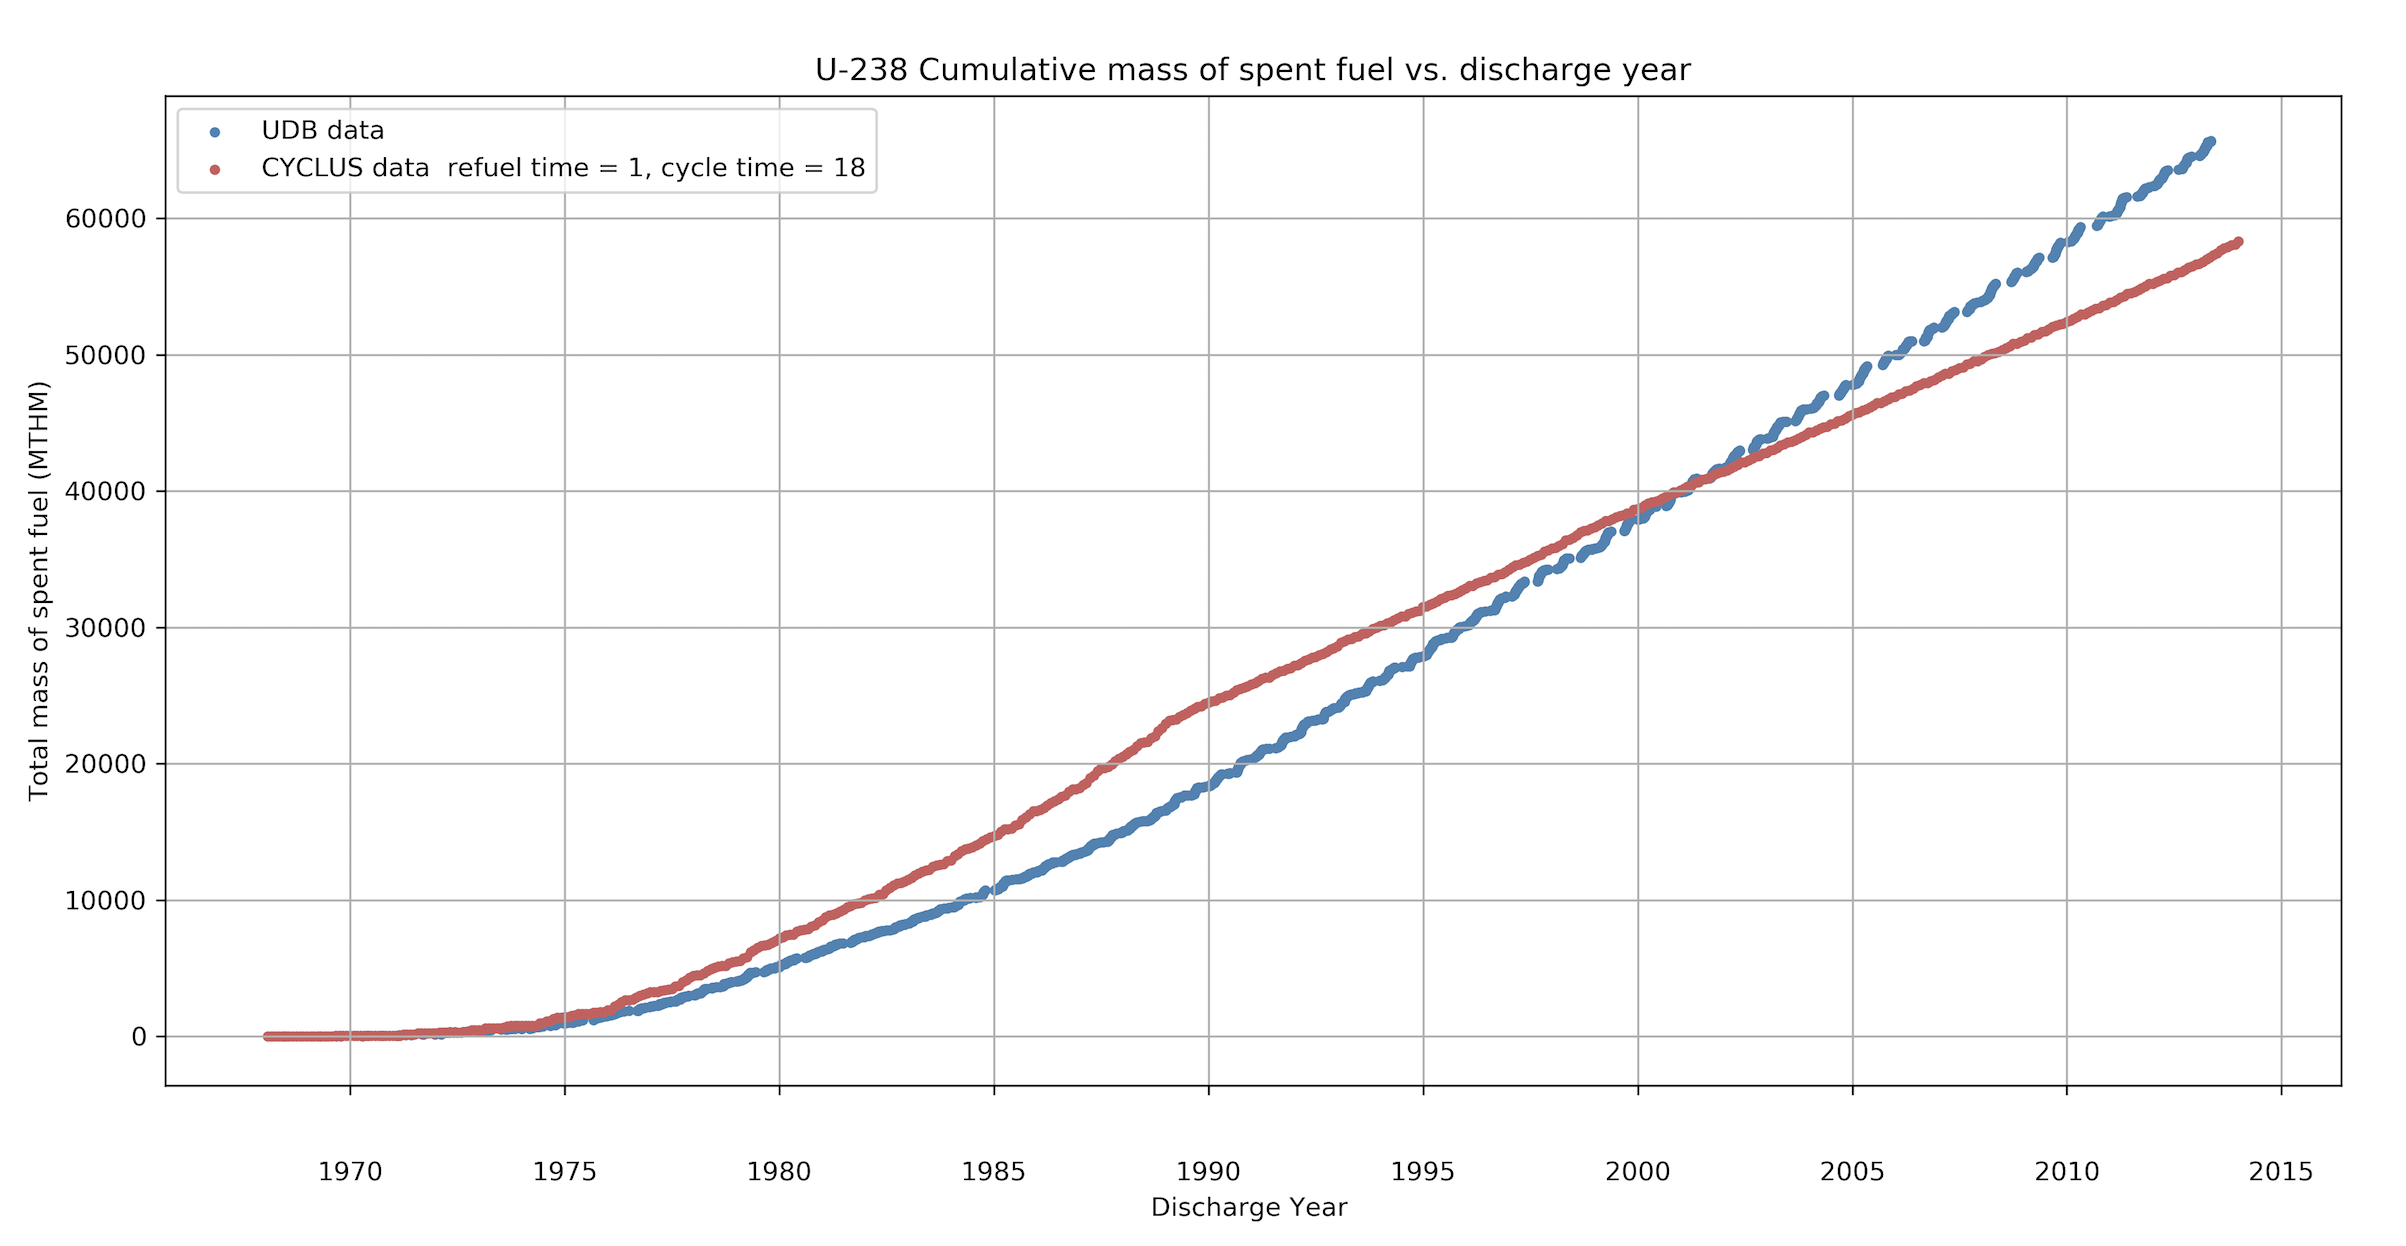
\includegraphics[width=\textwidth]{U-238_cumulative_mass_spent_fuel_original}
		\caption[Network2]%
		{{\small Total cumulative U-238 mass in spent fuel against discharge time for \Cyclus and UDB from 1967 to 2013}}    
		\label{fig:total_u238}
	\end{subfigure}
	\hfill
	\begin{subfigure}[b]{0.45\textwidth}  
		\centering 
		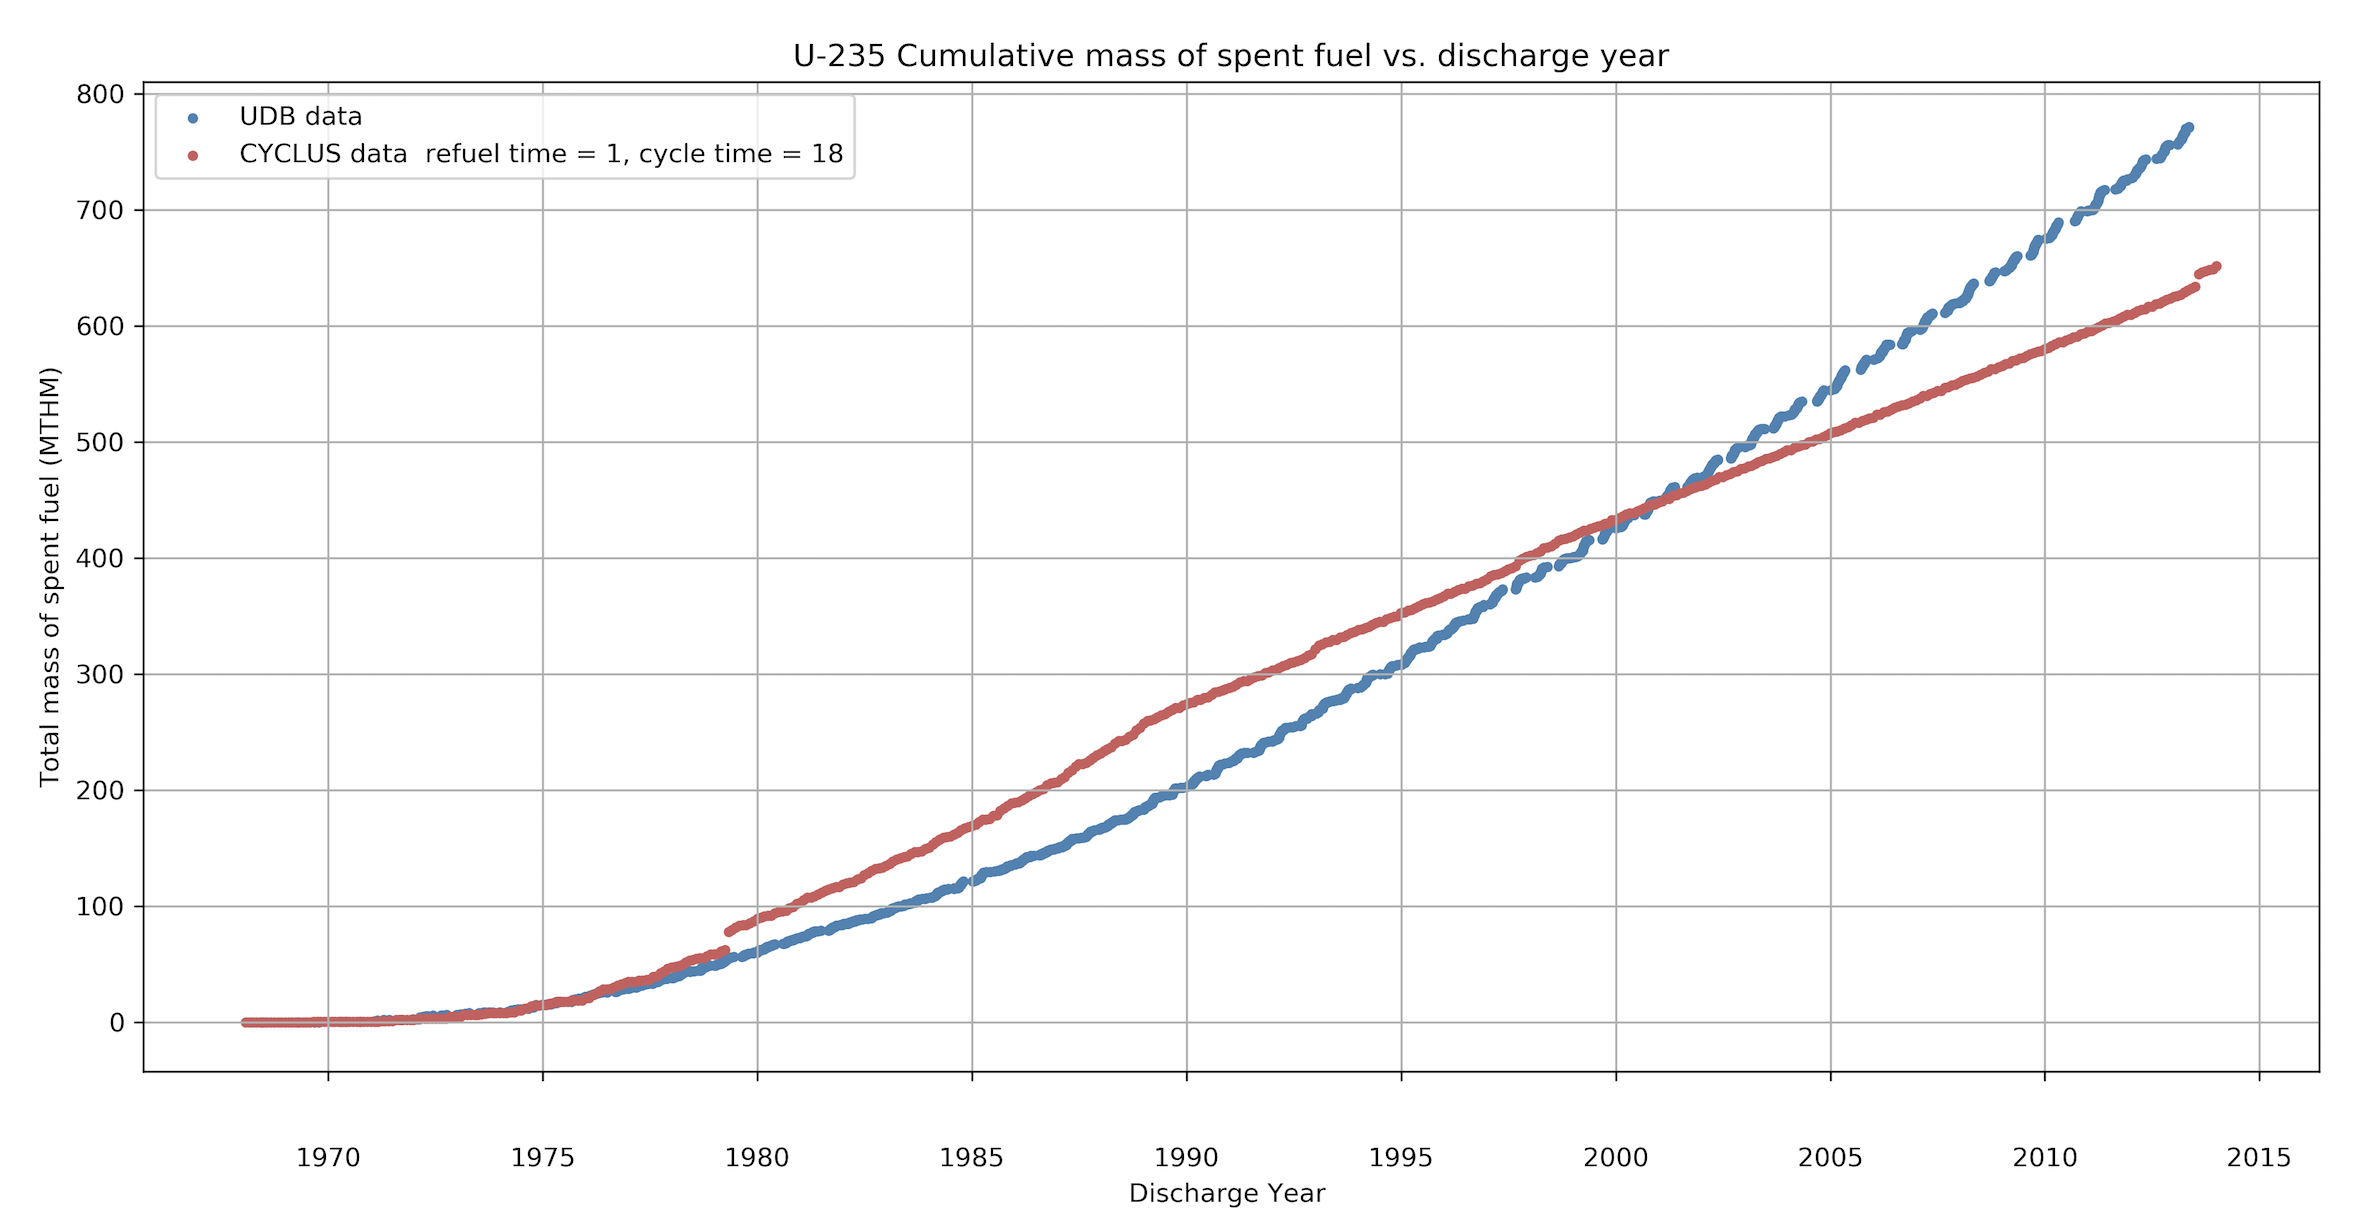
\includegraphics[width=\textwidth]{U-235_cumulative_mass_spent_fuel_original}
		\caption[]%
		{{\small Total cumulative U-235 mass in spent fuel against discharge time for \Cyclus and UDB from 1967 to 2013}}    
		\label{fig:total_u235}
	\end{subfigure}
	\vskip\baselineskip
	\begin{subfigure}[b]{0.45\textwidth}   
		\centering 
		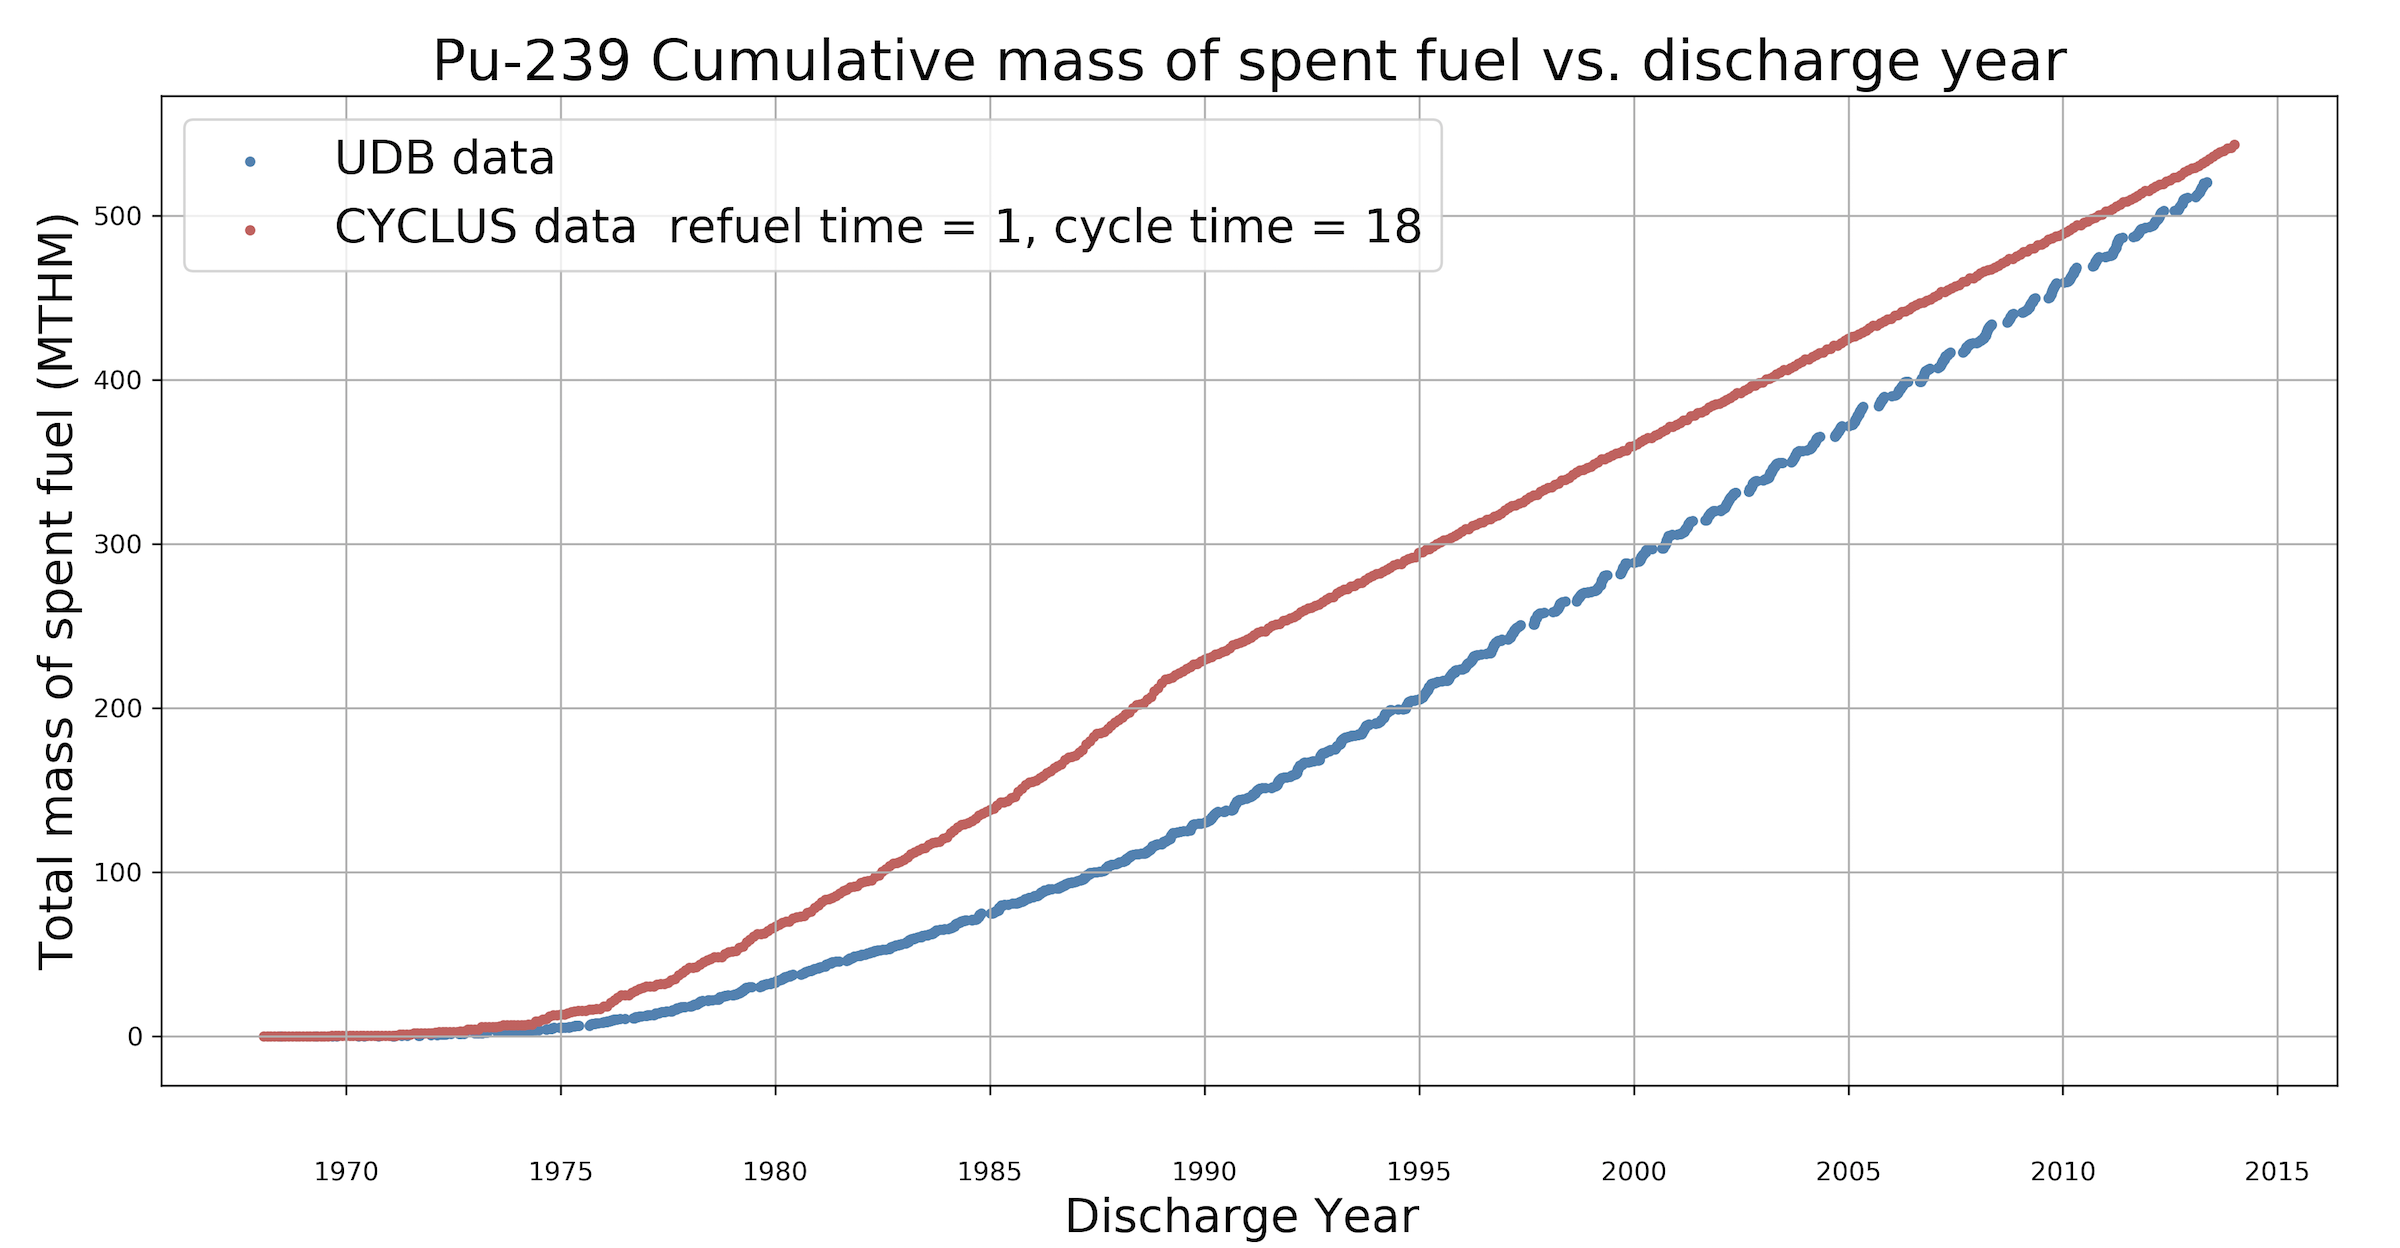
\includegraphics[width=\textwidth]{Pu-239_cumulative_mass_spent_fuel_original}
		\caption[]%
		{{\small Total cumulative Pu-239 mass in spent fuel against discharge time for \Cyclus and UDB from 1967 to 2013}}    
		\label{fig:total_pu240}
	\end{subfigure}
\caption{Total cumulative masses for specific isotopes in spent fuel against discharge time for \Cyclus and UDB from 1967 to 2013}
\end{figure}

%%%%%%%%%%%%%%%%%%%%%%%%%%%%%%%%%%%%%%%%%%%%%%%%%%%%%%%%%%%%%%%%%%%%%%%%%%%%%%%%
\section{Conclusions}
This work demonstrates that the spent fuel mass and isotopic composition results from the \Cyclus simulation of the United States nuclear fuel cycle closely follow the results from real world metrics. This proves that these results can be used to produce accurate isotopic decay heat contributions and simulate loading of a waste repository based on thermal constraints. However, improvements can be made to more closely replicate reality.  

Further work that can improve the simulation is to give the reactor agent the capability to accept varying cycle and refuel times. Therefore, by looking at the historic United States reactor operating data, a \Cyclus simulation can be made to replicate their cycle and refuel times even more closely. This would give more accurate spent fuel mass and isotopic compositions which will in turn make the simulations for loading of a waste repository more accurate. 

%%%%%%%%%%%%%%%%%%%%%%%%%%%%%%%%%%%%%%%%%%%%%%%%%%%%%%%%%%%%%%%%%%%%%%%%%%%%%%%%
\section{Acknowledgments}
This research is being performed using funding received from the DOE Office of Nuclear Energy's
Nuclear Energy University Program (Project 16-10512) "Demand-Driven Cycamore Archetypes". The authors want to thank members of the Advanced Reactors and Fuel Cycles research group (ARFC) at University of Illinois at Urbana Champaign in particular Jin Whan Bae for valuable advice and Gregory Westphal for proofreading. We also thank our colleagues from the \Cyclus community, particularly those in the University of Wisconsin Computational Nuclear Engineering Research Group (CNERG) and the University of South Carolina Energy Research Group (ERGS) who provided collaborative support in the development of the core software, \Cyclus, enabling this work. 

%%%%%%%%%%%%%%%%%%%%%%%%%%%%%%%%%%%%%%%%%%%%%%%%%%%%%%%%%%%%%%%%%%%%%%%%%%%%%%%%
\bibliographystyle{ans}
\bibliography{bibliography}
\end{document}

